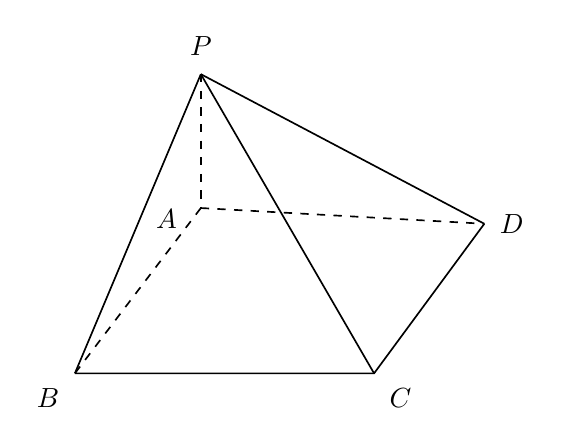
\begin{tikzpicture}[line width=.6pt]
\coordinate (P) at (0,3.2);
\coordinate (A) at (0,1.5);
\coordinate (B) at (-1.6,-0.6);
\coordinate (C) at (2.2,-0.6);
\coordinate (D) at (3.6,1.3);
% base
\draw (B)--(C)--(D);
\draw[dashed] (A)--(D);
\draw[dashed] (A)--(B);
% height + laterals
\draw[dashed] (P)--(A);
\draw (P)--(B);
\draw (P)--(C);
\draw (P)--(D);
% labels
\node[above=3pt] at (P) {$P$};
\node[below left=2pt,xshift=-3pt,yshift=5pt] at (A) {$A$};
\node[below left=2pt] at (B) {$B$};
\node[below right=2pt] at (C) {$C$};
\node[right=2pt] at (D) {$D$};
\end{tikzpicture}
